\section{SEAS problems}
\subsection{Modeling Environment}
The applications are motivated by the study of quasi-static deformation of the solid Earth over the time scales of earthquake cycles.
In both the interseismic and coseismic phases, the off-fault material response is modeled as elastic-plastic.
\begin{equation}\label{eqn:governing}
    \rho \ddot{u} = \nabla \cdot \sigma + F, \sigma = \boldsymbol{C} : (\epsilon - \epsilon^p) 
\end{equation}

Here, $\rho$ is the material density, $u$ is the vector of particle displacements, $F$ is the body fordce, $\boldsymbol{C}$ is the stiffness tensor of elastic moduli, and $\epsilon$ and $\epsilon^p$ are the elastic and plastic strains.
\begin{figure}
    \centering
    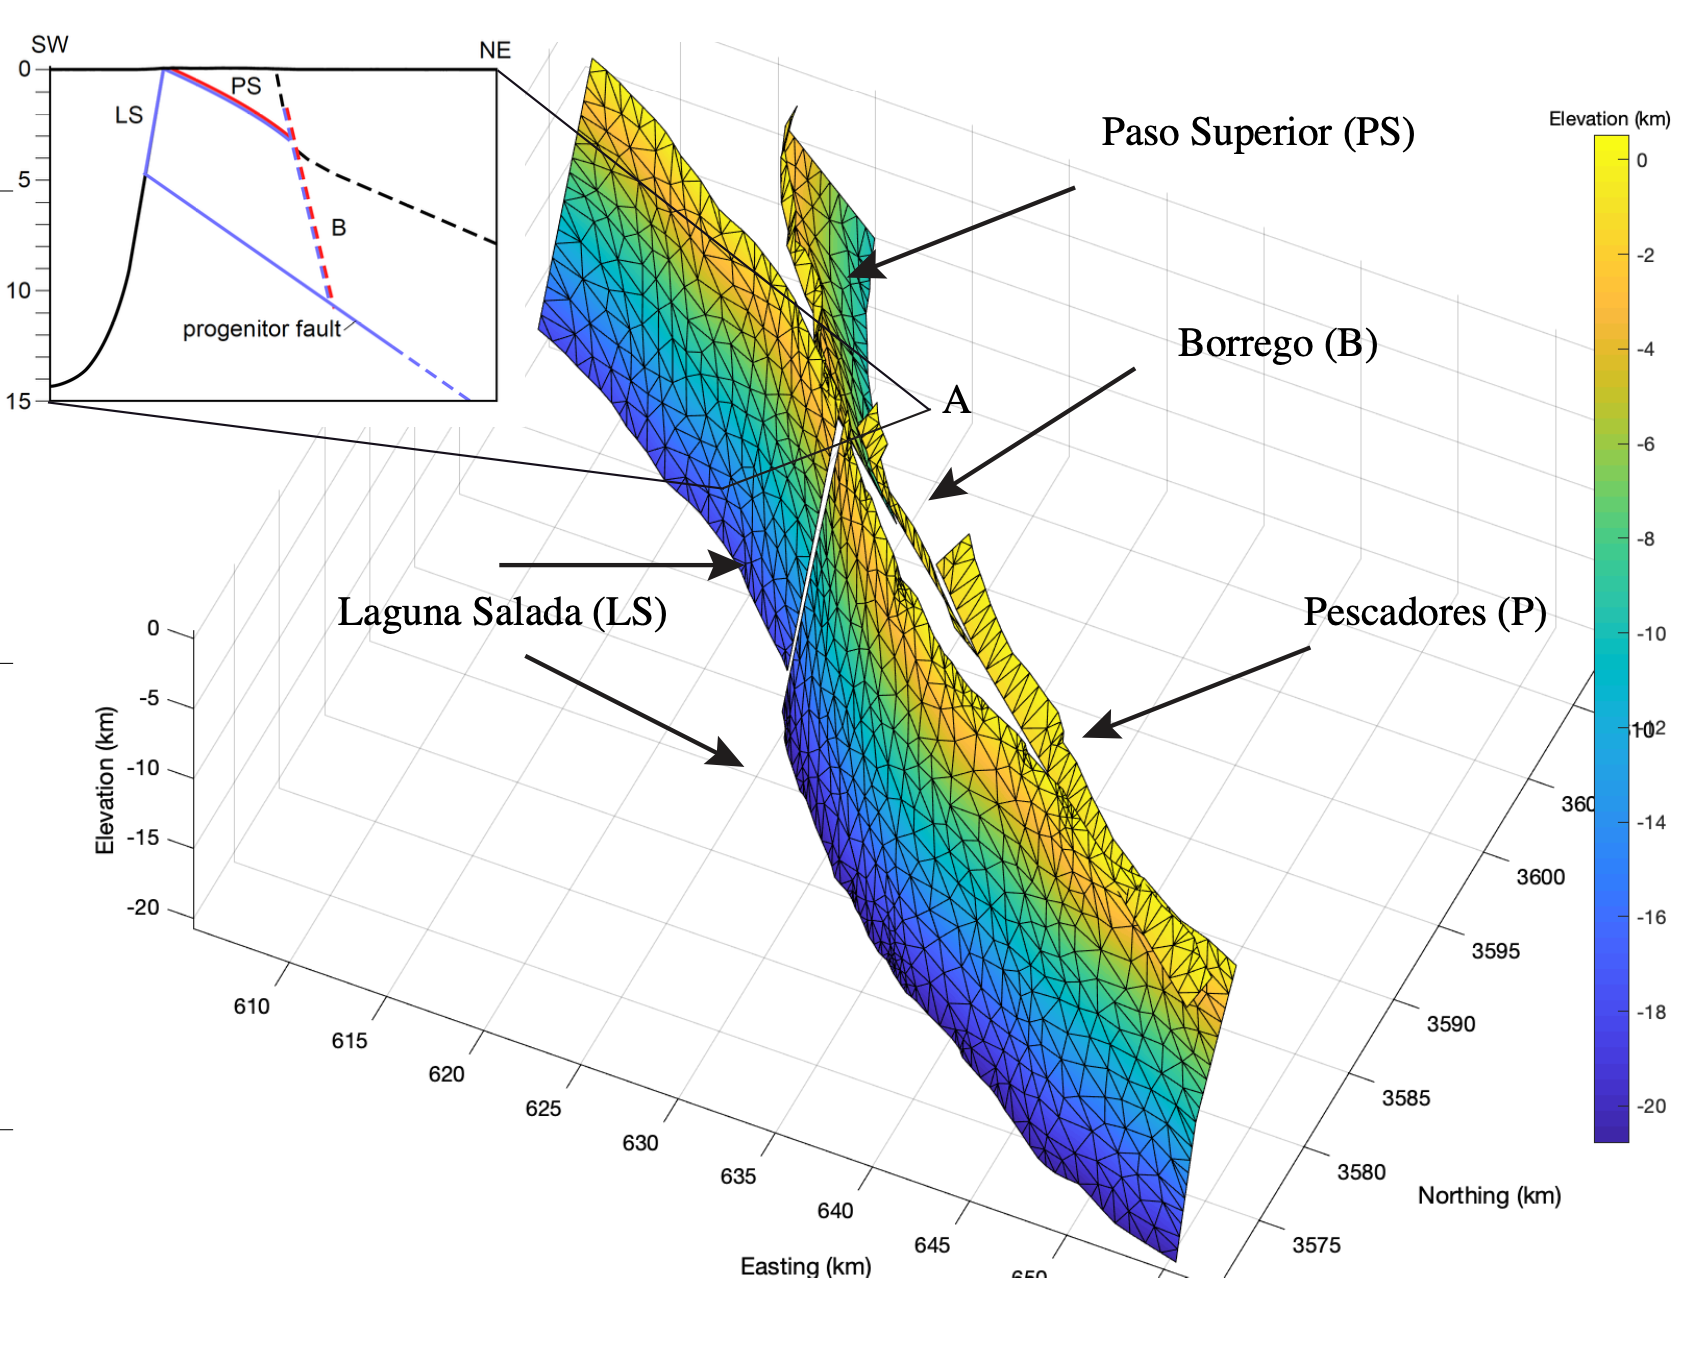
\includegraphics[width=\linewidth]{figures/fault-network.png}
    \caption{A 3D image of the complex fault network from EMC earthquake; image generated using scripts from \cite{https://doi.org/10.1002/2016GL072289}}
    \label{fig:fault-network}
\end{figure}
A fault network (shown in Figure \ref{fig:fault-network}) is composed of faults governed by non-linear, rate-and-state friction which determines the relationship between the slip velocity $V$ to shear traction $\tau$ with the (effective) norm stress $\bar{\sigma}$, the friction coefficient $f$ and a state variable $\Psi$.
\begin{equation}\label{eqn:friction-law}
    \tau = \bar{\sigma} f(V,\Psi), \Psi = G(V, \Psi)
\end{equation}
The form of the state evolution law $G$ can take several forms such as the aging law in which the state evolves in the absence of slip or the slip law with strong rate-weakening.

During the interseismic phase, the inertial terms in the governing equation \ref{eqn:governing} are set 0 ($\ddot{u} = 0$).
Tectonic loading is imposed through time-dependent boundary conditions and the slip on faults are incorporated through friction law \ref{eqn:friction-law}.
The evolution of $\Psi$ constraints the time step, and very large time steps can be used during the interseismic phase.
The main computational challenge comes from solving the large linear systems of equations that come from the discretization of the steady-state version of the equation \ref{eqn:governing}.
During the interseismic phase, tectonic loading determines the boundary conditions and the stress on faults as the result of elastic deformation.
Once an event begins to nucleate, we enter the coseismic phase and inertial terms of governing equation \ref{eqn:governing} are retained.
It is more efficient to use explicit integration during this period because it simplifies the computation. In both phases, the governing equation can be solved using the SBP-SAT methods mentioned in the previous section.

\subsection{3D Problem Setup}
The 3D problem setup described below is taken from previous SEAS publications \cite{10.1785/0220190248}.
The medium is assumed to be a homogeneous, isotropic, linear elastic half-space defined by
\begin{equation} \label{eqn:domain}
    \textbf{x} = (x_1, x_2, x_3) \in (-\infty, \infty) \times (\infty, \infty) \times (0, \infty)
\end{equation}

with a free surface at $x_3 = 0$ and $x_3$ as positive downward. A vertical, strike-slip fault is embedded at $x_1 = 0$, We use the notation ``+'' and ``-'' to refer to the different sides of the fault. 

We assume 3D motion, letting $u_i = u_i(\textbf{x}, t), i = 1, 2, 3$ denote the displacement in the $i$-direction.

Hooke’s law for linear elasticity is given by
\begin{equation}
    \sigma_{ij} = K\epsilon_{kk}\delta_{ij} + 2\mu (\epsilon_{ij} - \frac{1}{3} \epsilon_{kk}\delta_{ij})
\end{equation}
for bulk modulus $K$ and shear modulus $\mu$. The strain-displacement relations are given by 
\begin{equation}
    \epsilon_{ij} = \frac{1}{2} \left[\frac{\partial u_i}{\partial x_j} + \frac{\partial u_j}{\partial x_i}\right]
\end{equation}

The description of these benchmark problems can be found in \cite{erickson2018seas,jiang2020seas}.

To simulate the SEAS problems using the quasi-static method, it usually follows these steps.

\begin{algorithm}
    \caption{Quasi-static Formulation Algorithm}
    \begin{algorithmic}[1]
        \State \textbf{Step 1:} Initialize boundary conditions and state variables
        
        \While{simulation time not reached}
            \State \textbf{Step 2:} Solve steady-state problems to obtain displacements
            \State \hspace{1em} In 2D, Solve Poisson's equation
            \State \hspace{1em} In 3D Solve linear elasticity
            
            \State \textbf{Step 3:} Calculate stress from displacements
            
            \State \textbf{Step 4:} Calculate displacement velocity using stress and rate-and-state frictions
            
            \State \textbf{Step 5:} Determine time step size ($dt$) using ODE solver
            
            \State \textbf{Step 6:} Calculate state variables using aging law and $dt$
            
            \State \textbf{Step 7:} Update boundary conditions using velocity and $dt$
        \EndWhile
    \end{algorithmic}
\end{algorithm}

The DifferentialEquations.jl package provides powerful adapted ODE solvers based on Runge-Kutta methods and useful ODE interfaces that allow us to modify data and write to outputs.
The key challenge here is step 2 which requires solving a large linear system that is formed with the SBP-SAT methods.
It's difficult to apply direct methods due to their high memory requirements and computational inefficiency. 
In the next two chapters, we will go into detail to first formulate the linear systems using the SBP-SAT methods and then apply HPC algorithms to solve such problems.